\documentclass[a4paper]{article} 
\addtolength{\hoffset}{-2.25cm}
\addtolength{\textwidth}{4.5cm}
\addtolength{\voffset}{-3.25cm}
\addtolength{\textheight}{5cm}
\setlength{\parskip}{0pt}
\setlength{\parindent}{0in}

\usepackage{natbib}
\usepackage{blindtext} % Package to generate dummy text
\usepackage{charter} % Use the Charter font
\usepackage[utf8]{inputenc} % Use UTF-8 encoding
\usepackage{microtype} % Slightly tweak font spacing for aesthetics
\usepackage{amsthm, amsmath, amssymb} % Mathematical typesetting
\usepackage{float} % Improved interface for floating objects
\usepackage{hyperref} % For hyperlinks in the PDF
\usepackage{graphicx, multicol} % Enhanced support for graphics
\usepackage{xcolor} % Driver-independent color extensions
\usepackage{pseudocode} % Environment for specifying algorithms in a natural way
\usepackage[ddmmyyyy]{datetime} % Uses YEAR-MONTH-DAY format for dates
%\usepackage{gensymb}
\usepackage{bibentry}

\usepackage{fancyhdr} % Headers and footers
\pagestyle{fancy} % All pages have headers and footers
\fancyhead{}\renewcommand{\headrulewidth}{0pt} % Blank out the default header
\fancyfoot[L]{} % Custom footer text
\fancyfoot[C]{} % Custom footer text
\fancyfoot[R]{\thepage} % Custom footer text
\newcommand{\note}[1]{\marginpar{\scriptsize \textcolor{red}{#1}}} % Enables comments in red on margin

%----------------------------------------------------------------------------------------

\usepackage{adjustbox}
\usepackage{float}
\usepackage{multicol}
\usepackage{pgfplots, pgfplotstable}
\usepackage[european]{circuitikz}
%-------------------------------
%	TITLE VARIABLES (identify your work!)
%-------------------------------

\newcommand{\yourname}{Jakob Kralj 4.A} % replace YOURNAME with your name
\newcommand{\papertitle}{Zaporedna vezava uporanikov} % replace X with paper title

\begin{document}

%-------------------------------
%	TITLE SECTION (do not modify unless you really need to)
%-------------------------------
\fancyhead[C]{}
\hrule \medskip
\begin{minipage}{0.295\textwidth} 
\raggedright
\footnotesize
\yourname \hfill\\ 
\end{minipage}
\begin{minipage}{0.69\textwidth} 
\centering 
\Large
\text{\papertitle}\\ 
\normalsize 
\end{minipage}
\medskip\hrule 
\bigskip


%-------------------------------
%	ASSIGNMENT CONTENT (add your responses)
%-------------------------------

\section*{Naloga:} % this is an example

Ugotovi, kako se porazdelijo napetosti pri zaporedni vezavi upornikov.

\section*{Potrebščine:}

ŠMI, žice, trije voltmetri, plošča, kocke za sestavljanje električnega kroga.

\section*{Skica:}
\begin{center}
\begin{circuitikz}
\draw
(0,0) -- (0,2)
  to[resistor, l=$R_{1} {=}100\Omega $] (4,2) to[resistor, l=$R_{2} {=}500\Omega $]
  (8,2) -- (8,0)
  to[battery] (0,0)
  (2.5,0) -- (2.5,-1)
  to[voltmeter, l_=$U_0$] (5.5,-1) -- (5.5,0)
  (1,2) -- (1,4)
  to[voltmeter, l=$U_1$] (3,4) -- (3,2)
  (5,2) -- (5,4)
  to[voltmeter, l=$U_2$] (7,4) -- (7,2)
;
\end{circuitikz}
\end{center}
\section*{Meritve:}

Vezje z dvema zaporedno vezanima upornikoma priključi na ŠMI. Spreminjaj napetost vira ter meri napetost na upornikih ter na viru. Opravi vsaj pet meritev. Meritve vpisuj v tabele.

\begin{table}[H]
   \centering
\begin{tabular}{llll}
   $U_0[V]$ & $U_1[V]$ & $U_2[V]$ & $U_1 : U_2$ \\
   1 & 0,20 & 0,90 & 1:4 \\
   2 & 0,40 & 1,65 & 1:4,1 \\
   3 & 0,52 & 3,50 & 1:4,8 \\
   4 & 0,70 & 3,40 & 1:4,9 \\
   5 & 0,88 & 4,20 & 1:4,8
\end{tabular}
\end{table}



\section*{Rezultati in Interpretacija:}

$U_1$ in $U_2$ se večinoma skupaj seštejeta v napetost vira $U_0$, kjer se razmerje napetosti razdeli razmerju uporov. 
Teoretične vrednosti v realnem svetu ne moremo doseči zaradi prenizke notranje upornosti voltmetra, izgubah na žicah in nenatančnega odčitavanja vrednosti. 


\section*{Dodatek}
Zaporedno vezanima upornikoma vzporedno veži še en upornik. Pri izbrani napetosti vira (do 20V) izračunaj napetosti na posameznih upornikih. Izračunane vrednosti preveri še z meritvami.
\subsection*{Skica}

\begin{center}
   \begin{circuitikz}
   \draw
   (0,0) -- (0,2)
     to[resistor, l=$R_{1} {=}100\Omega $] (4,2) to[resistor, l=$R_{2} {=}500\Omega $]
     (8,2) -- (8,0)
     to[battery] (0,0)
     (2.5,0) -- (2.5,-1)
     to[voltmeter, l_=$U_0 {=} 5V$] (5.5,-1) -- (5.5,0)
     (1,2) -- (1,4)
     to[voltmeter, l=$U_1$] (3,4) -- (3,2)
     (5,2) -- (5,4)
     to[voltmeter, l=$U_2$] (7,4) -- (7,2)
     (0,2) -- (0,6) to[resistor, l=$R_{3} {=}100\Omega $] (8,6) -- (8,2)
     (2,6) -- (2,8) to[voltmeter, l=$U_1$] (6,8) -- (6,6)
   ;
   \end{circuitikz}
\end{center}

\subsection*{Izračun}
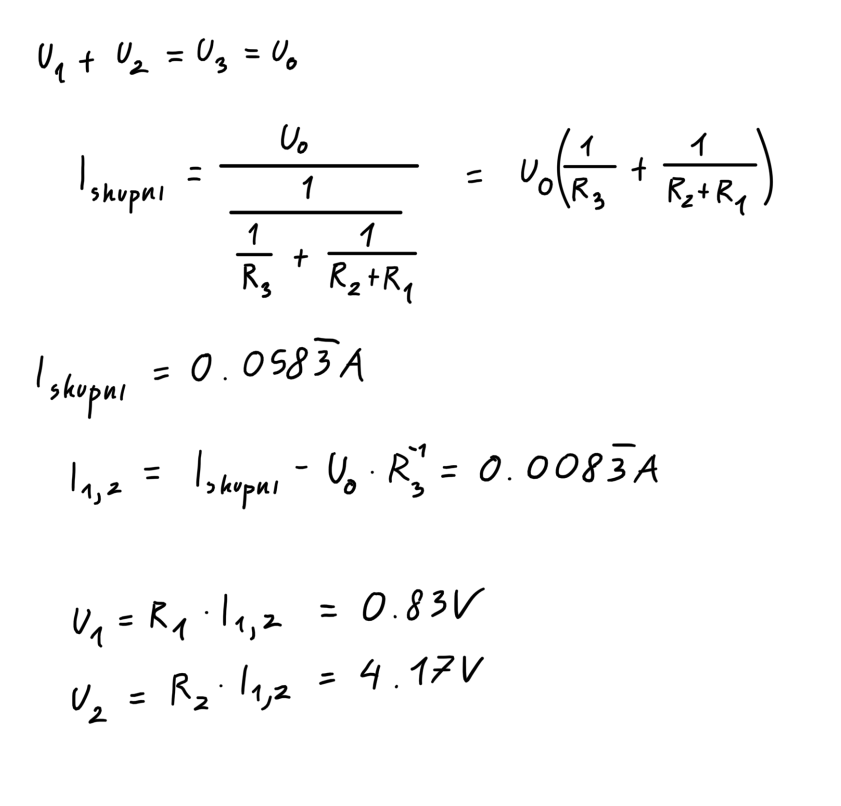
\includegraphics[scale=0.6]{racun.png}
\subsection*{Meritve}
\begin{gather}
   U_1 = 0.8V \\
   U_2 = 4,1V \\
   U_3 = 5V \\
\end{gather}
\end{document}